\newpage
\newcommand{\tab}{\hspace*{4em}}
\begin{appendix}
\section{Appendix}
\subsection{The Post-Study System Usability Questionnaire Items}
{\parindent0pt

1. Overall, I am satisfied with how easy it is to use this system.

STRONGLY AGREE\tab\tab\tab\tab\tab STRONGLY DISAGREE\\
\\
\tab1\tab2\tab3\tab4\tab5\tab6\tab7\tab8\tab\tab N/A\\
\\
Comments:.........................................................................................................................................\\
\\
\\
2. It was simple to use this system.

STRONGLY AGREE\tab\tab\tab\tab\tab STRONGLY DISAGREE\\
\\
\tab1\tab2\tab3\tab4\tab5\tab6\tab7\tab8\tab\tab N/A\\
\\
Comments:.........................................................................................................................................\\
\\
\\
3. I could effectively complete the tasks and scenarios using this system.

STRONGLY AGREE\tab\tab\tab\tab\tab STRONGLY DISAGREE\\
\\
\tab1\tab2\tab3\tab4\tab5\tab6\tab7\tab8\tab\tab N/A\\
\\
Comments:.........................................................................................................................................\\
\\
\\
4. I was able to complete the tasks and scenarios quickly using this system.

STRONGLY AGREE\tab\tab\tab\tab\tab STRONGLY DISAGREE\\
\\
\tab1\tab2\tab3\tab4\tab5\tab6\tab7\tab8\tab\tab N/A\\
\\
Comments:.........................................................................................................................................\\
\\
\\
5. I was able to efficiently complete the tasks and scenarios using this system.

STRONGLY AGREE\tab\tab\tab\tab\tab STRONGLY DISAGREE\\
\\
\tab1\tab2\tab3\tab4\tab5\tab6\tab7\tab8\tab\tab N/A\\
\\
Comments:.........................................................................................................................................\\
\\
\\
6. I felt comfortable using this system.

STRONGLY AGREE\tab\tab\tab\tab\tab STRONGLY DISAGREE\\
\\
\tab1\tab2\tab3\tab4\tab5\tab6\tab7\tab8\tab\tab N/A\\
\\
Comments:.........................................................................................................................................\\
\\
\\
7. It was easy to learn to use this system.

STRONGLY AGREE\tab\tab\tab\tab\tab STRONGLY DISAGREE\\
\\
\tab1\tab2\tab3\tab4\tab5\tab6\tab7\tab8\tab\tab N/A\\
\\
Comments:.........................................................................................................................................\\
\\
\\
8. I believe I could become productive quickly using this system.

STRONGLY AGREE\tab\tab\tab\tab\tab STRONGLY DISAGREE\\
\\
\tab1\tab2\tab3\tab4\tab5\tab6\tab7\tab8\tab\tab N/A\\
\\
Comments:.........................................................................................................................................\\
\\
\\
Note: The “interface” includes those items that you use to interact with the system. For example, some components of the interface are the keyboard, the mouse, the microphone, and the screens (including their use of graphics and language).\\
\\
9. The interface of this system was pleasant.

STRONGLY AGREE\tab\tab\tab\tab\tab STRONGLY DISAGREE\\
\\
\tab1\tab2\tab3\tab4\tab5\tab6\tab7\tab8\tab\tab N/A\\
\\
Comments:.........................................................................................................................................\\
\\
\\
10. I liked using the interface of this system.

STRONGLY AGREE\tab\tab\tab\tab\tab STRONGLY DISAGREE\\
\\
\tab1\tab2\tab3\tab4\tab5\tab6\tab7\tab8\tab\tab N/A\\
\\
Comments:.........................................................................................................................................\\
\\
\\
11. This system has all the functions and capabilities I expect it to have.

STRONGLY AGREE\tab\tab\tab\tab\tab STRONGLY DISAGREE\\
\\
\tab1\tab2\tab3\tab4\tab5\tab6\tab7\tab8\tab\tab N/A\\
\\
Comments:.........................................................................................................................................\\
\\
\\
12. Overall, I am satisfied with this system.

STRONGLY AGREE\tab\tab\tab\tab\tab STRONGLY DISAGREE\\
\\
\tab1\tab2\tab3\tab4\tab5\tab6\tab7\tab8\tab\tab N/A\\
\\
Comments:.........................................................................................................................................

\newpage
\subsection{Additional questionnaire}


Age: ............................................................................\\
\\
Gender: .........................................................................\\
\\
Study: ..........................................................................\\
\\
\\
1) How many hours per day do you use a keyboard \& mouse controlled device?\\
\\
......................................................................................................................................................................\\
\\
2) Did you use a LEAP motion before? (if so, for how many hours?)\\
\\
......................................................................................................................................................................\\
\\
3) What did you think of the experiment?\\
\\
......................................................................................................................................................................\\
\\
4) In which situation would you like to use the keyboard \& mouse?\\
\\
......................................................................................................................................................................\\
\\
5) In which situation would you NOT like to use the keyboard \& mouse?\\
\\
......................................................................................................................................................................\\
\\
6) In which situation would you like to use the LEAP motion?\\
\\
......................................................................................................................................................................\\
\\
7) In which situation would you NOT like to use the LEAP motion?\\
\\
......................................................................................................................................................................}

\newpage
\subsection{Models}\label{app:models}
\centerline{\begin{tabular}{m{4cm}m{4cm}m{4cm}m{4cm}}
\centerline{
\includegraphics{imgs/models/model1}}&\centerline{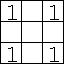
\includegraphics{imgs/models/model2}}&\centerline{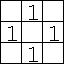
\includegraphics{imgs/models/model3}}&\centerline{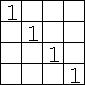
\includegraphics{imgs/models/model4}}\\
\centerline{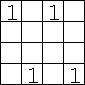
\includegraphics{imgs/models/model5}}&\centerline{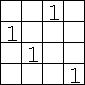
\includegraphics{imgs/models/model6}}&\centerline{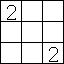
\includegraphics{imgs/models/model7}}&\centerline{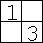
\includegraphics{imgs/models/model8}}\\
\centerline{
\includegraphics{imgs/models/model9}}&\centerline{
\includegraphics{imgs/models/model10}}&\centerline{
\includegraphics{imgs/models/model11}}&\centerline{
\includegraphics{imgs/models/model12}}\\
\centerline{
\includegraphics{imgs/models/model14}}&\centerline{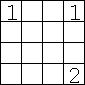
\includegraphics{imgs/models/model15}}&\centerline{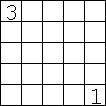
\includegraphics{imgs/models/model16}}&\centerline{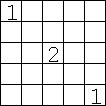
\includegraphics{imgs/models/model17}}\\
\centerline{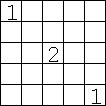
\includegraphics{imgs/models/model17}}&\centerline{
\includegraphics{imgs/models/model18}}&\centerline{
\includegraphics{imgs/models/model19}}&\centerline{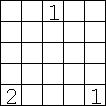
\includegraphics{imgs/models/model20}}
\end{tabular}}

\newpage
\subsection{Cognitive modeling: GOMS}
\begin{figure}[!htbp]
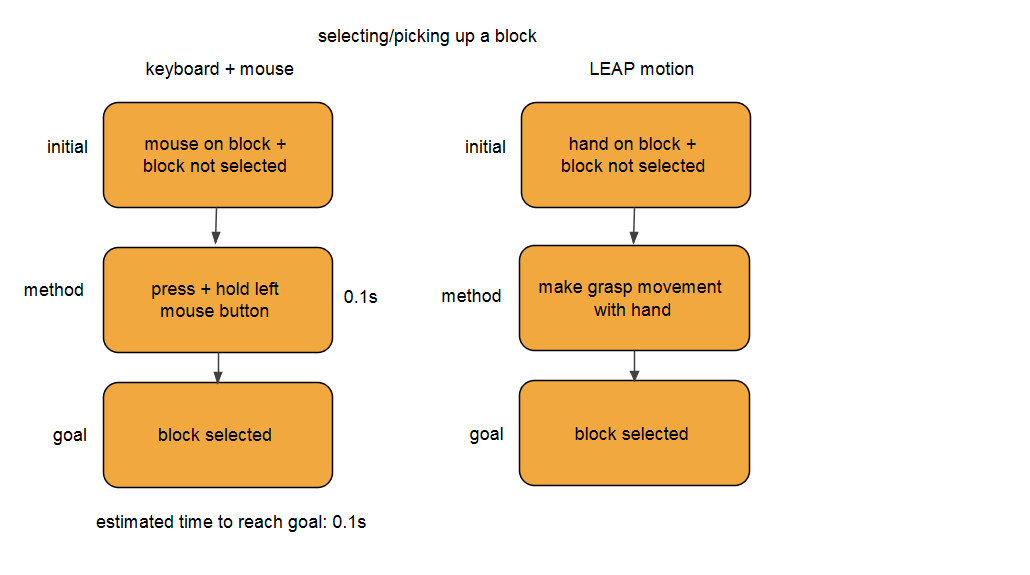
\includegraphics[width=\textwidth]{imgs/selectingblocks.png}
\caption{GOMS diagram for selecting a block.}
\label{fig:selectingblocks}
\end{figure}

\begin{figure}[!htbp]
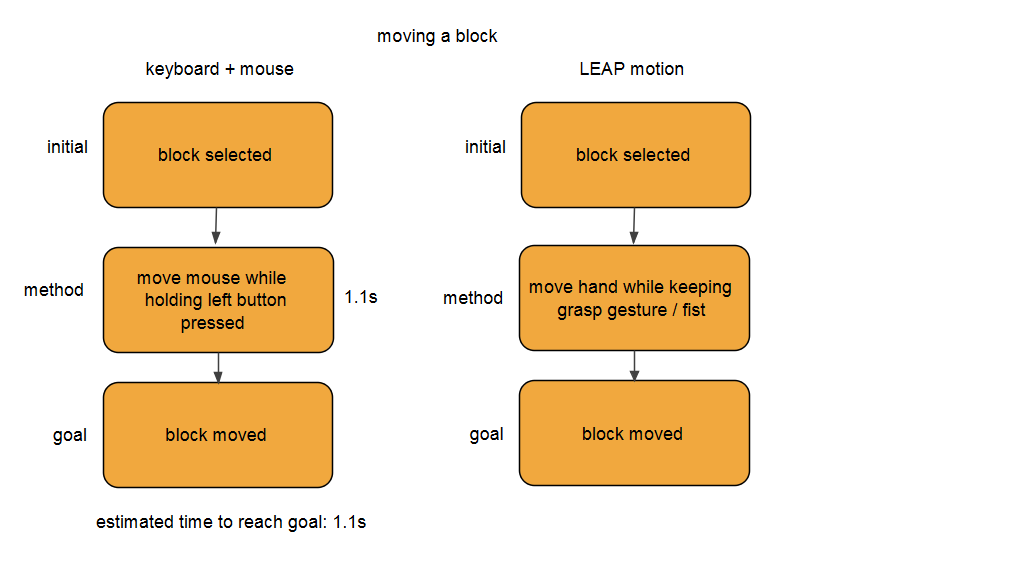
\includegraphics[width=\textwidth]{imgs/movingblock.png}
\caption{GOMS diagram for moving a block.}
\label{fig:movingblock}
\end{figure}

\begin{figure}[!htbp]
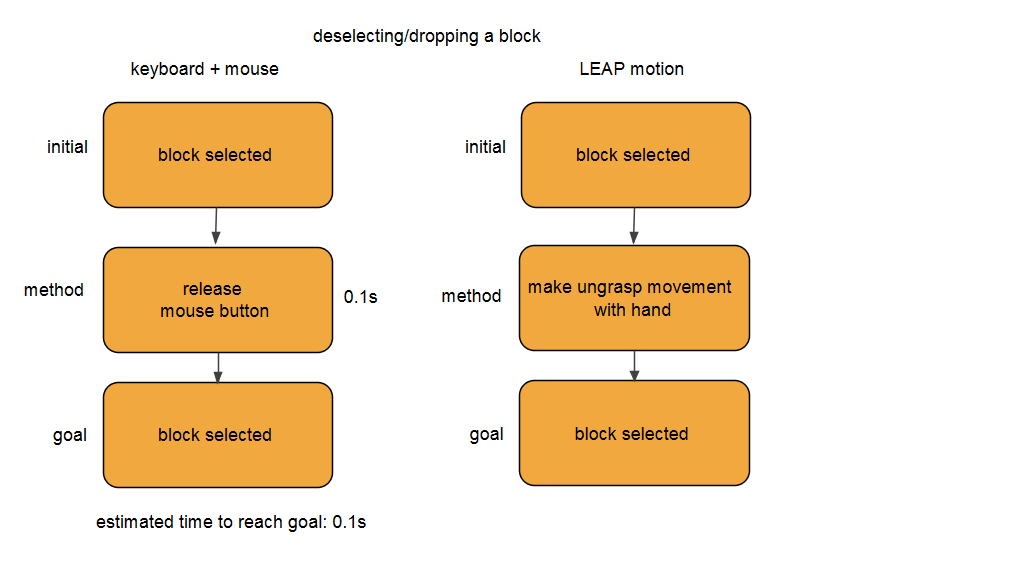
\includegraphics[width=\textwidth]{imgs/deselectingblocks.png}
\caption{GOMS diagram for deselecting a block.}
\label{fig:deselectingblocks}
\end{figure}

\begin{figure}[!htbp]
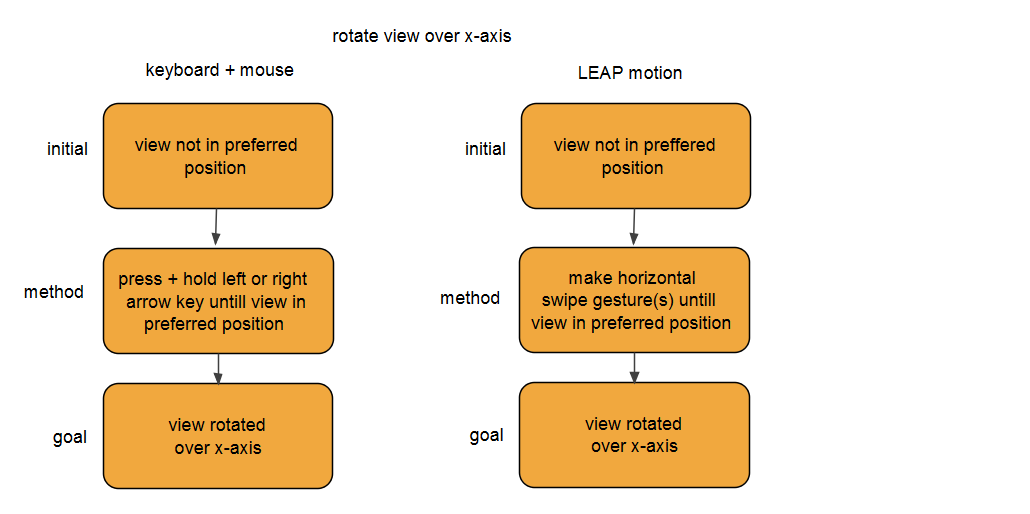
\includegraphics[width=\textwidth]{imgs/rotateviewx.png}
\caption{GOMS diagram for rotating the view in horizontal direction.}
\label{fig:rotateviewx}
\end{figure}

\begin{figure}[!htbp]
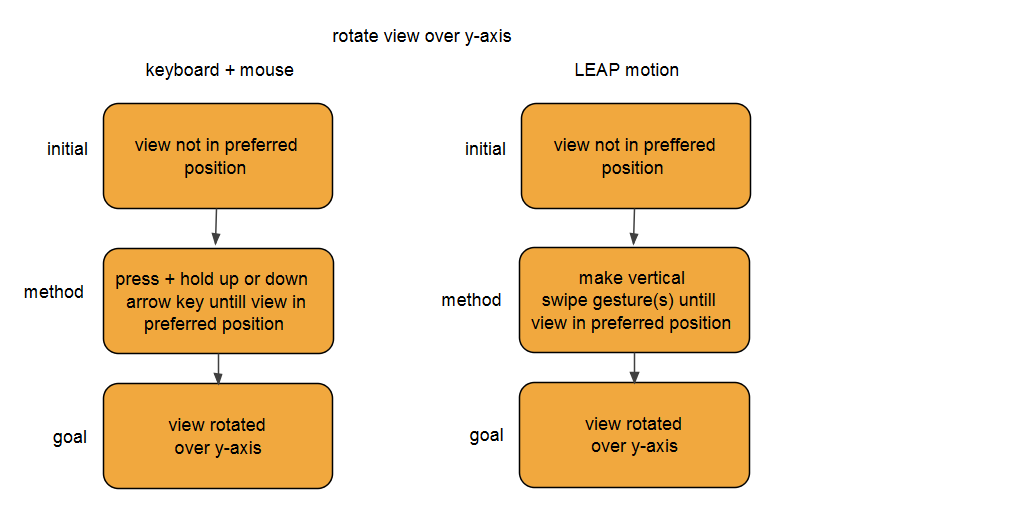
\includegraphics[width=\textwidth]{imgs/rotateviewy.png}
\caption{GOMS diagram for rotating the view in vertical direction.}
\label{fig:rotateviewy}
\end{figure}

\end{appendix}